\documentclass[runningheads,a4paper]{llncs}

\usepackage[american]{babel}

\usepackage{graphicx}
\usepackage{amssymb}
\usepackage[utf8]{inputenc}
\usepackage[T1]{fontenc}

%extended enumerate, such as \begin{compactenum}
\usepackage{paralist}

%put figures inside a text
%\usepackage{picins}
%use
%\piccaptioninside
%\piccaption{...}
%\parpic[r]{\includegraphics ...}
%Text...

%Sorts the citations in the brackets
%\usepackage{cite}

%for easy quotations: \enquote{text}
\usepackage{csquotes}

\usepackage[T1]{fontenc}

%enable margin kerning
\usepackage{microtype}

%better font, similar to the default springer font
\usepackage[%
rm={oldstyle=false,proportional=true},%
sf={oldstyle=false,proportional=true},%
tt={oldstyle=false,proportional=true,variable=true},%
qt=false%
]{cfr-lm}
%
%if more space is needed, exchange cfr-lm by mathptmx
%\usepackage{mathptmx}

%for demonstration purposes only
\usepackage[math]{blindtext}

\usepackage{multirow}
\usepackage[table,xcdraw]{xcolor}
\newcolumntype{M}[1]{>{\centering\arraybackslash}m{#1}}


\usepackage[
%pdfauthor={},
%pdfsubject={},
%pdftitle={},
%pdfkeywords={},
bookmarks=false,
breaklinks=true,
colorlinks=true,
linkcolor=black,
citecolor=black,
urlcolor=black,
%pdfstartpage=19,
pdfpagelayout=SinglePage
]{hyperref}
%enables correct jumping to figures when referencing
\usepackage[all]{hypcap}

\usepackage[inline]{enumitem}


\usepackage{enumitem}
\setlist[itemize,1]{label={\fontfamily{cmr}\fontencoding{T1}\selectfont\textbullet}}

\usepackage[capitalise,nameinlink]{cleveref}
%Nice formats for \cref
\crefname{section}{Sect.}{Sect.}
\Crefname{section}{Section}{Sections}
\crefname{figure}{Fig.}{Fig.}
\Crefname{figure}{Figure}{Figures}

\usepackage{amsmath}

%Table of contents
% make a proper TOC despite llncs
\setcounter{tocdepth}{3}
\makeatletter
\renewcommand*\l@author[2]{}
\renewcommand*\l@title[2]{}
\makeatletter




\usepackage{xspace}
\usepackage{cite}
%\newcommand{\eg}{e.\,g.\xspace}
%\newcommand{\ie}{i.\,e.\xspace}
\newcommand{\eg}{e.\,g.,\ }
\newcommand{\ie}{i.\,e.,\ }

\setcounter{secnumdepth}{3}

%introduce \powerset - hint by http://matheplanet.com/matheplanet/nuke/html/viewtopic.php?topic=136492&post_id=997377
\DeclareFontFamily{U}{MnSymbolC}{}
\DeclareSymbolFont{MnSyC}{U}{MnSymbolC}{m}{n}
\DeclareFontShape{U}{MnSymbolC}{m}{n}{
    <-6>  MnSymbolC5
   <6-7>  MnSymbolC6
   <7-8>  MnSymbolC7
   <8-9>  MnSymbolC8
   <9-10> MnSymbolC9
  <10-12> MnSymbolC10
  <12->   MnSymbolC12%
}{}
\DeclareMathSymbol{\powerset}{\mathord}{MnSyC}{180}

%improve wrapping of URLs - hint by http://tex.stackexchange.com/a/10419/9075
\makeatletter
\g@addto@macro{\UrlBreaks}{\UrlOrds}
\makeatother

% correct bad hyphenation here
\hyphenation{optical networks semiconductor}

\begin{document}

%Works on MiKTeX only
%hint by http://goemonx.blogspot.de/2012/01/pdflatex-ligaturen-und-copynpaste.html
%also http://tex.stackexchange.com/questions/4397/make-ligatures-in-linux-libertine-copyable-and-searchable
%This allows a copy'n'paste of the text from the paper
\input glyphtounicode.tex
\pdfgentounicode=1

\title{"Development of a new Information System for a Nonprofit Organization in the Cloud"}
%If Title is too long, use \titlerunning
%\titlerunning{Short Title}

%Single insitute
\author{Diogo André Cardoso Serafim\\
\textit{diogoserafim@tecnico.ulisboa.pt}
\\Advisor: José Borbinha 
\\Co-Advisor: Por definir}
%If there are too many authors, use \authorrunning
%\authorrunning{First Author et al.}
\institute{Instituto Superior Técnico}
\authorrunning{Cardoso Serafim et al.}


%Multiple insitutes
%Currently disabled
%
\iffalse
%Multiple institutes are typeset as follows:
\author{Firstname Lastname\inst{1} \and Firstname Lastname\inst{2} }
%If there are too many authors, use \authorrunning


\institute{
Insitute 1\\
\email{...}\and
Insitute 2\\
\email{...}
}
\fi
			
\maketitle


\begin{abstract}

\iffalse
Network security threats are becoming more and more proeminent and the connection links at ISPs are getting increasingly fast. Traditional network intrusion detection systems are either signature-based or behavior-based, which means looking up for known intrusion signatures in the packets, or detecting deviation from a normal behavior, respectively. With the exponential increase of network security threats, these IDSs are not able to cope with their growth, as they are only able to detect specific intrusions that are previously known. Also, most of them rely on payload inspection, that can be a bottleneck in the detection in real-time, and, now that almost every communication is done through encrypted messages, it is almost impossible to interpret the observed payload. In order to counter these limitations, our IDS will detect attacks using flows, which are defined as being a set of packets that passes a specific observation point in a given time period, with common characteristics. This work will therefore present a proposal for a flow-based IDS capable of detecting attacks without any \textit{a priori} knowledge, and therefore countering the limitations present in traditional IDSs. The results from this proposed system are to be validated with a real-world dataset provided by the Portuguese ISP Vodafone.
\fi
Este projeto consiste na elaboração de um sistema informático para uma associação sem fins lucrativos e de apoio social e ambiental. Surge da necessidade que a associação possui para a informatização dos seus processos atuais. Para o desenvolvimento do novo sistema é preciso, em primeiro lugar, efetuar um levantamento dos problemas que existem. Atualmente a associação gere todas as informações relativas aos seus beneficiários através de vários documentos em Excel. Isto resulta num sistema desatualizado, demorado e desordenado. Sé com a análise dos problemas que resultam do sistema atualmente utilizado, podemos obter uma melhor compreensão do seu funcionameto e quais as melhorias a introduzir. Esta proposta de solucão temo o objetivo de disponibilizar um sistema que reflita as etapas anteriores e adicione valor de negócio à associação. Estão refletidas as restrições do cliente, descreve os requisitos a considerar, apresenta uma arquitetura da solução e refere as principais preocupações a nível de seguraçaa do sistema. Finalmente atendendo às necessidades do cliente, e com base no método de desenvolvimento agil, apresenta-se um gráfico de Gantt que contem as fases de implementacao do projeto e a duracao do mesmo.
\end{abstract}

\keywords{Cloud Computing, Google, Authentication }
\let\cleardoublepage\relax
\tableofcontents
%%%%%%%%%%%%%%%%%%%%%%%%%%%%%%%%%%%%%%%%%%%%%%%%%%%%%%%%%%%%%%%%%%%%%%%%%%%%%%%
\section{Introduction}\label{sec:introduction}
%Works on MiKTeX only
%hint by http://goemonx.blogspot.de/2012/01/pdflatex-ligaturen-und-copynpaste.html
%also http://tex.stackexchange.com/questions/4397/make-ligatures-in-linux-libertine-copyable-and-searchable
%This allows a copy'n'paste of the text from the paper
\input glyphtounicode.tex
\pdfgentounicode=1

%Deixar para o fim. Apresentar uma introducao com base na relação entre cloud computing e nonprofit organizations

%%%%%%%%%%%%%%%%%%%%%%%%%%%%%%%%%%%%%%%%%%%%%%%%%%%%%%%%%%%%%%%%%%%%%%%%%%%%%%%
%\subsection{Animalife}\label{sec:related}
%%%%%%%%%%%%%%%%%%%%%%%%%%%%%%%%%%%%%%%%%%%%%%%%%%%%%%%%%%%%%%%%%%%%%%%%%%%%%%%
Animalife is a nonprofit organization of Social and Environmental Support, founded in October (2011). With headquarters set in Lisbon, this institution works in collaboration with more than 50 volunteers that dedicate much of their time supporting this social cause. The main goals of this institution are, the promotion of citizenship, environment protection, public health and protection of unemployed and disadvantaged people.

Animalife gives support in management and organization of other institutions responsible for the rescue of abandoned animals, taking care of them by promoting their vacination, deworming and sterilization and consequently the control of over-population of dogs and cats. 

It also conduct and support initiatives to improve the quality of life of families in need, through elimination of food shortages or other kind of pet animals that are in their care thus preventing the abandonment of animals and over-population in kennels and associations hostels.

%%%%%%%%%%%%%%%%%%%%%%%%%%%%%%%%%%%%%%%%%%%%%%%%%%%%%%%%%%%%%%%%%%%%%%%%%%%%%%%
\subsection{Motivation}\label{sec:related}
%%%%%%%%%%%%%%%%%%%%%%%%%%%%%%%%%%%%%%%%%%%%%%%%%%%%%%%%%%%%%%%%%%%%%%%%%%%%%%%
Deixar para o fim. Motivação do projeto de tese

%%%%%%%%%%%%%%%%%%%%%%%%%%%%%%%%%%%%%%%%%%%%%%%%%%%%%%%%%%%%%%%%%%%%%%%%%%%%%%%
\subsection{Problem Statement}\label{sec:related}
%%%%%%%%%%%%%%%%%%%%%%%%%%%%%%%%%%%%%%%%%%%%%%%%%%%%%%%%%%%%%%%%%%%%%%%%%%%%%%%

In terms of technology, Animalife works essentially with Microsoft Office Excel. Therefore, all the data relative to the families and animals is stored in spreadsheets. However, this information are spread over multiples documents leading to long and exhaustive operations. Thus, this problem aligned to the fact that the organization collects and records data in different ways according to the location, leads to an outdated system, compromising the performance and organization of the institution.\\

Taking in advance the general problem in providing database solutions to nonprofit organizations with limited resources and technical expertise, it is necessary to have a new information system in order to reduce the problems addressed above, maximizing productivity and organization of the institutions itself. So it is necessary to define a value proposition which would specify the benefits that Animalife will gain with this new system.

So according to all this aspects, the key points of the value proposition are as follows:
\begin{itemize}
\item Creation of a database solution that include data storage, easy access, manipulation, searching and storing capabilities in the cloud.
\item Creation of a new front-end layout for use by the volunteers.
\item Training materials for nonprofit volunteers.
\end{itemize}


%%%%%%%%%%%%%%%%%%%%%%%%%%%%%%%%%%%%%%%%%%%%%%%%%%%%%%%%%%%%%%%%%%%%%%%%%%%%%%%
\subsection{Document Structure}\label{sec:related}
%%%%%%%%%%%%%%%%%%%%%%%%%%%%%%%%%%%%%%%%%%%%%%%%%%%%%%%%%%%%%%%%%%%%%%%%%%%%%%%

This document is structured as follows:
\begin{itemize}
\item Section 2 aims to explore the relevant studies in cloud computing;
\item Section 3 provides the proposed solution of the architecture;
\item Section 4 provides the evaluation methods for the validation of the solution;   
\item Section 5 present a scheduling for the future work;
\item Section 6 presents some conclusions of this work.'
\end{itemize}
%%%%%%%%%%%%%%%%%%%%%%%%%%%%%%%%%%%%%%%%%%%%%%%%%%%%%%%%%%%%%%%%%%%%%%%%%%%%%%%

%%%%%%%%%%%%%%%%%%%%%%%%%%%%%%%%%%%%%%%%%%%%%%%%%%%%%%%%%%%%%%%%%%%%%%%%%%%%%%%

\section{Related Work}\label{sec:related}


%Works on MiKTeX only
%hint by http://goemonx.blogspot.de/2012/01/pdflatex-ligaturen-und-copynpaste.html
%also http://tex.stackexchange.com/questions/4397/make-ligatures-in-linux-libertine-copyable-and-searchable
%This allows a copy'n'paste of the text from the paper
\input glyphtounicode.tex
\pdfgentounicode=1

This section provides an overview of same major contributions in this area. Section 2.1 provides an insight about the core concepts of cloud computing, such as the architectural and business models of cloud computing. Section 2.2 describes some open standards related to the authentication and authorization protocols. Finally, Section 2.3 provides a comparison between the most known cloud storage providers and their services, including features and prices.
\subsection{Cloud Computing Core Concepts}\label{ssec:tools}
%%%%%%%%%%%%%%%%%%%%%%%%%%%%%%%%%%%%%%%%%%%%%%%%%%%%%%%%%%%%%%%%%%%%%%%%%%%%%%%

Described by the National Institute of Standards and Technology (NIST) as a {\it model for enabling convenient, on-demand network access to a shared pool of configurable computing resouces (e.g., networks, servers, storage, applications, and services) that can be rapidly provisioned and released with minimal management effort or service provider interaction}, \cite{Zhang2010}
cloud provides an architecture that can be divided into 4 layers: the hardware layer, the infrastructure layer, the platform and the application layer, as described bellow:

\begin{itemize}
\item \textit{The hardware layer}\\
Typically implemented in data centers, is responsible for managing the physical resources of the cloud, such as physical servers, routers, switches, power and cooling systems. Typical issues at hardware layer include hardware configuration, fault tolerance and traffic and power management.\cite{cloud:SS}\\

\item \textit{The infrastructure layer}\\
The infrastructure layer creates a pool of storage and computing resources by partitioning the physical resources using virtualization technologies (e.g., KVM, Xen, VMWare). It is an essential component of cloud computing since may key features are only available through virtualization technologies.\cite{cloud:SS} \\

\item \textit{The platform layer}\\
The platform layer is composed of the operating systems and application frameworks. Built on top of the infrastructure layer, the platform tries to minimize the load of deploying applications directly into VM containers. One of the best examples is the Google App Engine that operates at the platform layer to provide API support for implementing storage, database and business logic of typical web applications.\cite{cloud:SS}\\

\item \textit{The application layer}\\
Located at the the highest level of the hierarchy, the application layer consists of the actual cloud applications that make use of automatic-scaling feature to achieve better performance, availability and lower operating cost.\cite{cloud:SS}
\end{itemize}

Cloud computing also employs a service business model where hardware and platform-level resources are provided as services on-demand. In fact, every layer describe in the architecture can be implemented as a service to the layer below. Due to this fact, cloud offers services  that can be assigned to each layer, and grouped into three categories: infrastructure as a service (IaaS), platform as a service (PaaS) and software as a service (SaaS).


\begin{itemize}
\item \textit{IaaS - Infrastructure as a Servive }\\
It refers to on-demand provisioning of infrastructural resources i.e. users can subscribe to their favorite computing infrastructures with specified requirements in terms of hardware configuration, software installation and data access. Examples of IaaS providers include Amazon EC2 \cite{iaas:AmazonEC2} , GoGrid \cite{iaas:GoGrid} and Flexiscale\cite{iaas:FlexiScale}.  \\


\begin{figure}[h]
    \centering
    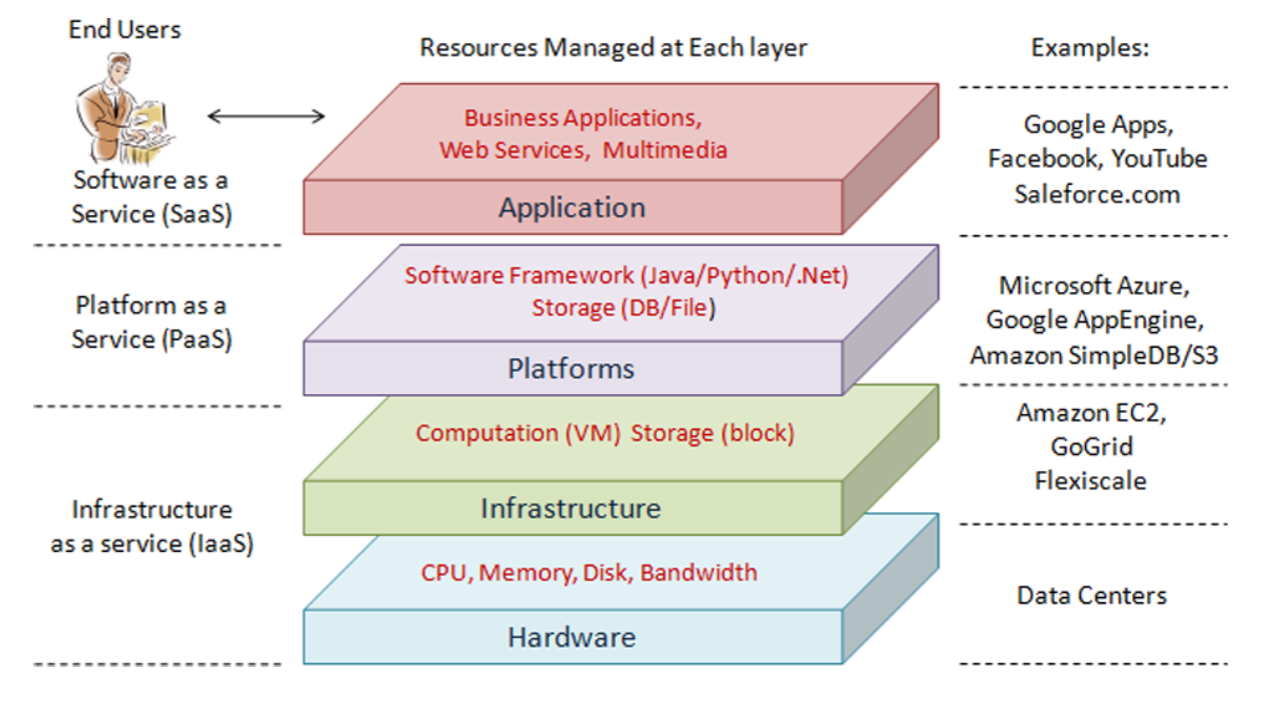
\includegraphics[width=\textwidth]{cloudArchitecture}
    \caption{Cloud Computing Architecture \cite{cloud:Archi}}
    \label{fig:cloudArchitecture}
\end{figure}

\item \textit{PaaS - Platform as a Servive }\\
It refers to the provisioning of platform software layer resources, including operating system support and software development frameworks. Examples of PaaS providers include Google App Engine, Microsoft Windows Azure and Force.com \cite{paas:Force}.\\

\item \textit{SaaS - Software as a Servive }\\
Software or an application is hosted as a service and provided to customers over the Internet. This is a very important service since it eliminates the need to install and run the application on the local computer. An important example of the SaaS is the Application Service Provider (ASP) whose main approach is to provide subscriptions to software that is hosted in the Internet. Google Chrome Browser is another example since it provides a desktop through which applications can be delivered locally or remotely, in addition to the traditional web browsing experience. Another examples include SalesForce.com and Rackspace \cite{saas:RackSpace}\\
\end{itemize}


\subsection{Web Authentication \& Authorization Open Technology}\label{ssec:security}


\begin{itemize}
\item {\it OpenID -} is an open standard for user authentication that allows the use of an existing account to sign in to multiple websites, without needing to create new passwords. It offers the possibility to associate information ( such as name or email address) with user's OpenID, that can be shared with the websites visited.

\begin{figure}[h]
    \centering
    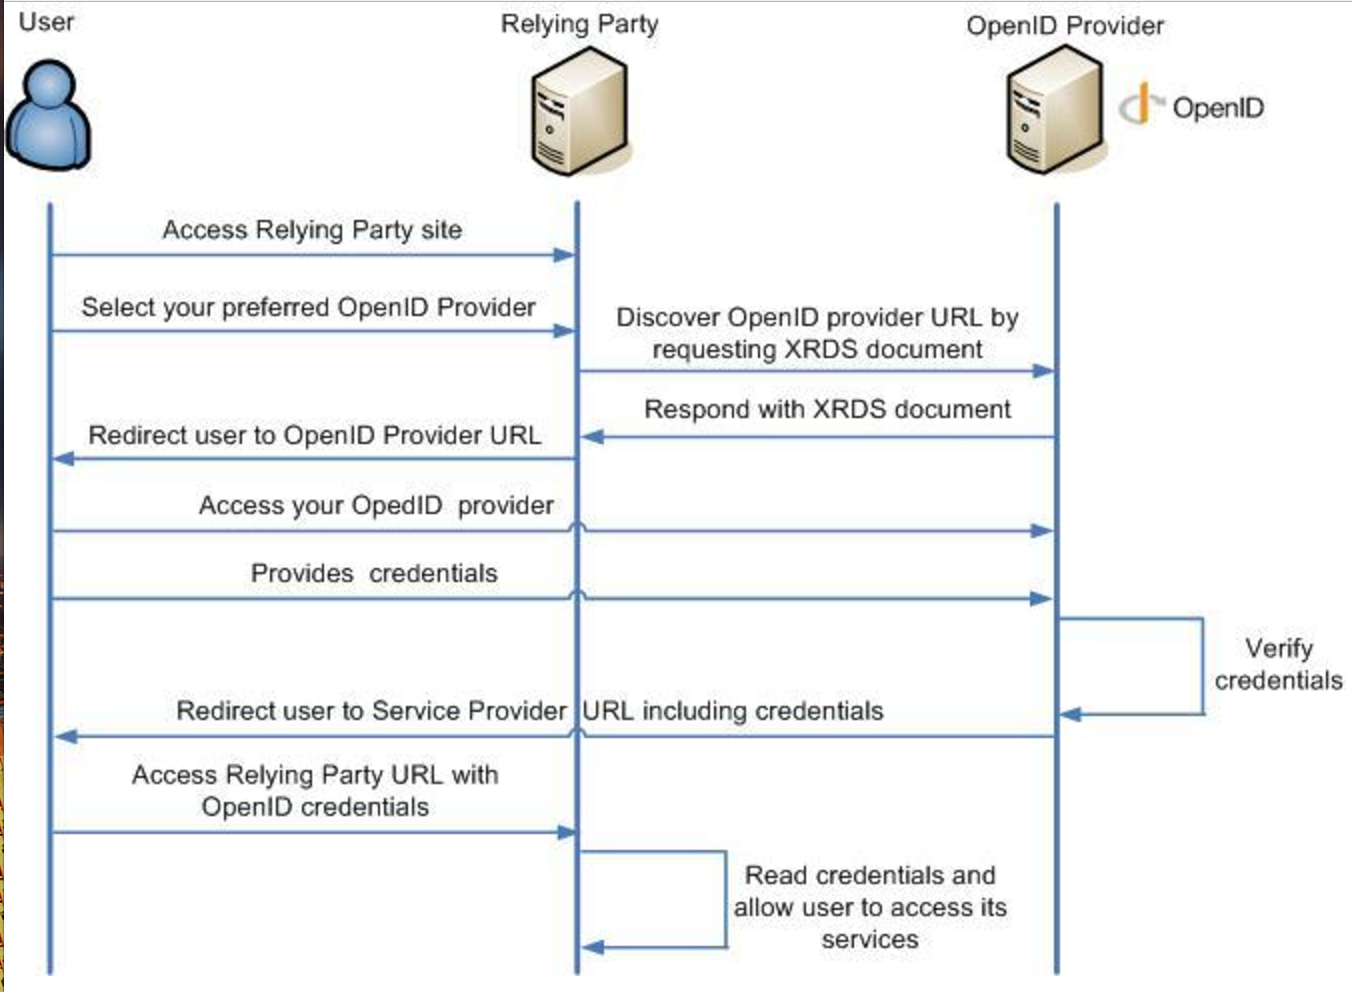
\includegraphics[width=1.0\textwidth]{openID}
    \caption{OpenID Authentication Flow}
    \label{fig:openID}
\end{figure}
%(citar o openID http://openid.net/get-an-openid/what-is-openid/).
To do that OpenID provides a framework for communication between the identity provider and the relying party. The user may have an account or multiple accounts with a specified identity provider, and then use this identity to authenticate to any service that accepts OpenID authentication. 

The flow process of OpenID comprises three entities: the user, the relying party which wants to verify the user identity and an entity provider that provides the OpenID URLs as despicted in figure \ref{fig:openID}.\\

With OpenID the user's password is only given to the identity provider and this one confirms the identity to the websites visited so, no website sees the password. Therefore, it is considered as safe since it not compromises the user's identity by some kind of insecure websites.\cite{cloud:openID}\\


\item {\it Shibboleth -} is another open standard, similar to OpenID, whose main approach is to manage single sign on (SSO), allowing users to authenticate to different services using just one piece of information.
Shibboleth is an open source implementation of federated identity based management, where the identity providers provide information and the service providers consume this information giving access to content or services. %{\textbf CITAR https://shibboleth.net/about/}. 

A user authenticates with his organizational credentials, and the organization (or identity provider) passes the minimal identity information necessary to the service provider to enable an authorization decision. It also provides extended privacy functionality allowing a user to control the attributes released to each application.\\ %{\textbf CITAR 15\\}


\item {\it OAuth - } is an open standard that provides a solution for internet users to authorize websites or applications to access their information, without sharing their credentials such as passwords or usernames.%\textbf {CITAR: Whitson Gordon. "Understanding OAuth: What Happens When You Log Into a Site with Google, Twitter, or Facebook". Retrieved 2016-05-15.}
Designed to work specifically with Hypertext Transfer Protocol (HTTP), it allows access tokens to be issued to third-party clients by an authorization server, with the approval of the resource owner. The third party then uses the access token to access the protected resources hosted by the resource server. %\textbf{CITAR: "RFC 6749 - The OAuth 2.0 Authorization Framework". Retrieved 2016-05-15.}

\begin{figure}[h]
    \centering
    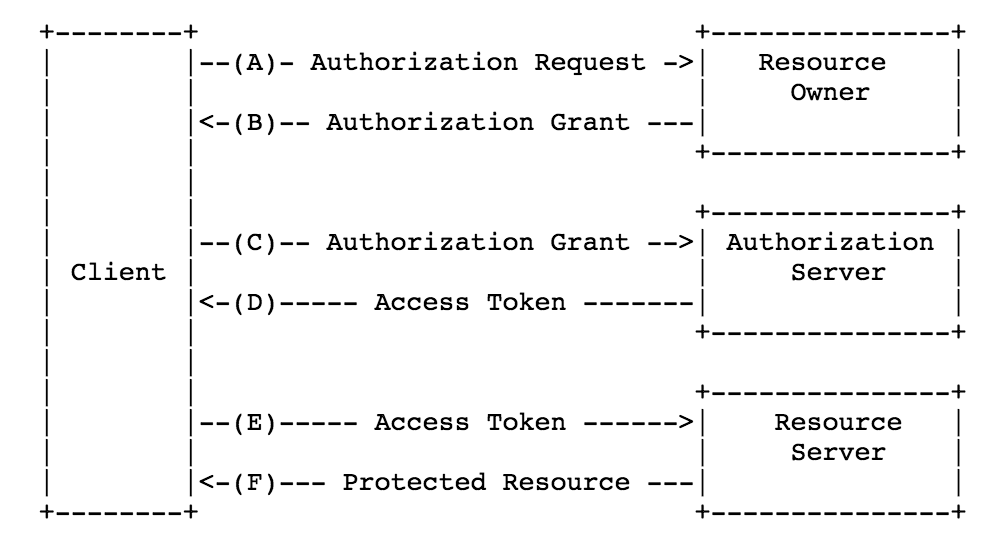
\includegraphics[width=1.0\textwidth]{OAuth}
    \caption{OAuth Protocol flow}
    \label{fig:OAuth}
\end{figure}

Since the creation, OAuth is being used by many social networking websites for authorization of various applications. Once the permissions are granted the application is able to download the complete stream of social data agains the user which is then kept for data mining purposes.% \textbf{CITAR O PAPER}.
More than a protocol, it is a framework is interoperable with any newer version of itself (e.g. Auth2.0).   
\end{itemize}

\subsection{Cloud Providers}\label{ssec:storage}

The industry of cloud storage has lot of potential in terms of growth of storage and faster retrieval. When organizations call for certain services offered by Cloud Storage Providers (CSPs), it is implicit that the they will choose the CSP that best suits the requirements of such organization. CSPs are also defined as Hosts, responsible for keeping the data available and accessible in a physical environment protected and running. People and organizations buy or lease storage capacity from the storage provider in order to store user, organization, or application data. Cloud storage Services may be accessed through cloud computer service, a web service application programming interface (API) or by applications that utilize the API, such as cloud desktop storage, a cloud storage gateway \cite{cloud:cloudStorageGateway} or Web-based content management systems.

Many cloud storage services offers a free account with some limitations, such as the amount of storage provided (usually from 2GB up to 5GB), or a file size limit for upload. 
An overview of the services  of the dominant Cloud Providers in the industry and their services is given bellow. 

\begin{enumerate}
\item {\it Amazon Cloud Drive -}
Amazon Cloud Drive is a cloud storage application managed by Amazon that offers secure cloud storage, file backup, file sharing and photo printing. Acting like a personal hard drive in the cloud, it can be accessed through multiple devices and offers 2 types of plans: one enables user with an unlimited storage for photos and the other one offers a 5GB of cloud storage space free of cost in a three-month trial.
There is no limit for the number of files to be uploaded, but each file needs to be under 2GB.

The advantage of Amazon Cloud Drive resides on the fact that if the user already have an Amazon account, doesn't need to sign up for a new service.
However, unlike other cloud storage services, the desktop app just allows the user to upload or download files, and can only view or manage files from the cloud drive website.\\

\item {\it Dropbox -}
Dropbox is one of the most used cloud storage services, allowing the store of any kind of file in the cloud. With Dropbox, users can easily move files from their computers to the cloud and vice versa by dragging and dropping them into the Dropbox folder.
The service automatically and quickly syncs files across all the devices registered for a specified account, available everywhere and independent from the device that it is being used. 
There is no size limit on file upload, but larger files can take several hours to upload, depending on network connection speed.
As an advantage, Dropbox gives its users a lot of opportunities to get extra storage (despite the 2GB offered through the sign up). If the user participate in the quick Getting Started Tutorial, the space increases more 250MB. Turn on the automatic photo upload feature on any of the mobile apps allows more 3GB of extra space. It's also possible to earn 500MB for each friend referred to Dropbox if it actually signs up for the service, up to 16GB total, or 32 referrals.
However, the website does not allow user to control how files are displayed.\\

\item {\it Box -}
Box is another cloud storage service that also provides sharing and privacy features for business and users. Beyond the basic cloud storage setup, where it's possible to store any kind of file, Box lets users to share files between them, assign tasks, leave comments on someone's work and get notifications when a file changes. User can also preview files from Box website and even create simple text documents. Like other cloud storage services box gives a lot of control over the privacy of a file, allowing user to decide who can view and open specific folders and files. It also allows user to define passwords for his files and set expiration dates for shared folders.
One of biggest advantages of Box is that, it allows business users to connect 
other apps, such as Salesforce and NetSuite \cite{cloud:netSuite}, so that you can easily save documents to Box. There are also plug-ins for Microsoft Office and Adobe Lightroom that let the user open and edit files saved to Box from those applications.

However The service's endless list of sharing and privacy features can be lost on someone who's just using the service for personal storage.
Because of all those features, it can feel overwhelming to navigate the Box website if you're only trying to manage a few files and folders.\\

\item {\it Microsoft OneDrive -}
OneDrive is a cloud storage service provided by Microsoft, that allows the store of any kind of file in the service, including photos, video and documents, and then access them from any Windows desktop or mobile device. One of the most important strengths of OneDrive, is that it works closely with Microsoft Office apps (e.g. Office 365). Therefore, anyone that has an Office 365 subscription will have access to OneDrive, collaborating with other people in real time.

In late 2015, Microsoft made an announcement that it would no longer offer unlimited cloud storage to Office 365 subscribers. Instead, subscribers are limited to 1TB. In the case of OneDrive Storage plans it offers a 50GB for \$1.99 per month plan (besides the 5GB offered initially to anyone that has a Microsoft Account). 
Another disadvantage of OneDrive resides on the fact that, the automatic file organization not always put files in the correct folders.\\

\item {\it Google Drive -}
Google Drive is the cloud storage service created by Google. Released on April 2012, allows users to store files in the cloud, synchronize files across devices and share files. It also combines a complete set of office tools such Google Docs, Sheets and Slides in an office suite that provides collaborative editing of documents, spreadsheets and presentations.
For those who have a Google account, it's easy to access google drive and enable the service in seconds. However, the 15GB initially provided are shared with other services such as Gmail (it's possible to save attachments from the e-mail directly to drive), and Google+. Like the other cloud providers, google drive can be accessed through a web browser or desktop app, but unfortunately if the user uses Google Drive tools to create documents, spreadsheets or presents, it must export those files to edit them in another program.
\end{enumerate}
The following table provides an overview of all the cloud providers described above and makes a comparison between them in terms of file size restriction, free storage, the possibility of earn extra storage, the paid plans that are available in the market and specific costs and the operative systems that supports each kind of service.
\begin{center}
\begin{tabular}{ |M{2.5cm}|M{2cm}|M{2cm}|M{2cm}|M{2cm}|M{2cm}|M{2cm}| }
 \hline
 \multicolumn{6}{|c|}{\textbf{Cloud Providers Comparison}} \\
 \hline
 & \textbf{OneDrive} & \textbf{Dropbox} & \textbf{Google Drive} & \textbf{Box} & \textbf{Amazon Cloud Drive}\\
 \hline
 \textbf{File Size Restriction} & 10GB&10GB with website, none with Dropbox apps&5TB&250MB for free plan, 5GB for paid personal plan&2GB*\\  \hline
 \textbf{Free storage} & 5GB&2GB&15GB&10GB&No**\\  \hline
 \textbf{Earn extra free storage} & No & Yes & No & No & No\\ \hline
 \textbf{Paid Plans} & €2/month for 50GB & €8.25/month for 1TB, €10/month unlimited storage for business teams (each user)	& €2/month 100GB, €10/month for 1TB up to 30TB of storage & €10/month for 100GB & €10.99/year for unlimited photos, €60/year for unlimited storage\\ \hline
 \textbf{OSes supported}	 & Windows, Mac, Android, iOS, Windows Phone	& Windows, Mac, Linux, Android, iOS, Windows Phone, BlackBerry, Kindle Fire	&Windows, Mac, Android, iOS	&Windows, Mac, Android, iOS, Windows Phone, BlackBerry	& Windows, Mac, Android, iOS, Kindle Fire.
\\
 \hline
\end{tabular}
*There is no file size limit with desktop apps.\\
**Amazon Cloud Drive offers limited free storage with an Amazon Prime subscription.
\end{center}





%%%%%%%%%%%%%%%%%%%%%%%%%%%%%%%%%%%%%%%%%%%%%%%%%%%%%%%%%%%%%%%%%%%%%%%%%%%%%%%

\section{Google API em Detalhe}\label{sec:proposal}

%
%Works on MiKTeX only
%hint by http://goemonx.blogspot.de/2012/01/pdflatex-ligaturen-und-copynpaste.html
%also http://tex.stackexchange.com/questions/4397/make-ligatures-in-linux-libertine-copyable-and-searchable
%This allows a copy'n'paste of the text from the paper
\input glyphtounicode.tex
\pdfgentounicode=1

This section provides an overview of same major contributions in this area. Section 2.1 provides an insight about the functional aspects of cloud, such as the architectural, business and various operation models of cloud computing. Section 2.2 describes some open standards related to the authentication and authorization protocols . Section 2.3 provides a brief introduction of the various cloud service providers and their services. FALTA COMPLETAR.... 
\section{Google em detalhe}
\section{Guidelines/Agile profile para fazer um protocolo web}\label{ssec:tools}




\subsection{Class Diagram}
\subsection{Functional Requirements}
\subsection{Technologies}
\subsubsection{Google API}
\subsubsection{Google API Spreadsheet}
\subsubsection{Node.js}
\subsubsection{Angular.js}



%%%%%%%%%%%%%%%%%%%%%%%%%%%%%%%%%%%%%%%%%%%%%%%%%%%%%%%%%%%%%%%%%%%%%%%%%%%%%%%

\section{Methodologies and Best Practices for Software Development}\label{sec:proposal}

%Works on MiKTeX only
%hint by http://goemonx.blogspot.de/2012/01/pdflatex-ligaturen-und-copynpaste.html
%also http://tex.stackexchange.com/questions/4397/make-ligatures-in-linux-libertine-copyable-and-searchable
%This allows a copy'n'paste of the text from the paper
\input glyphtounicode.tex
\pdfgentounicode=1

In the past years, organizations have seen changes in the field of software development when it comes to implementation models and related processes. Constant changes, especially in requirements become difficult when more rigid software processes are applied. Slowness to accommodate uncertainty and rapid changes inevitably lead to obsolescence of software and customer dissatisfaction \cite{agile:1}. Changes in requirements may turn software artifacts already planned, designed, specified and even already implemented in obsolete and outdated artifacts.
It is desirable that software processes have sufficient flexibility to accommodate inevitable changes and uncertainties. At the same time, it is expectable that these processes might be described, monitored and improved.
For that reason one of the most important approaches for software development in the last years is the use of development methodologies. 

There are two types of methodologies: Waterfall and Agile. The Waterfall method is one of the oldest product development models. The success of the model in delivering a robust, high quality product has been well documented. Agile methods were developed to overcome the limitations of traditional software development methods such waterfall method.

This section describes the best methodology approaches for software development including their benefits and challenges when applied to different scenarios. 

\subsection{Waterfall Methodology}

Waterfall is a sequential model where the software development lifecycle is divided into 5 phases: (1) Requirement Analysis, (2) Design (3) Implementation (4) Verification (5) Maintenance, with each phase having its own tasks and goals. 

\begin{figure}[h]
    \centering
    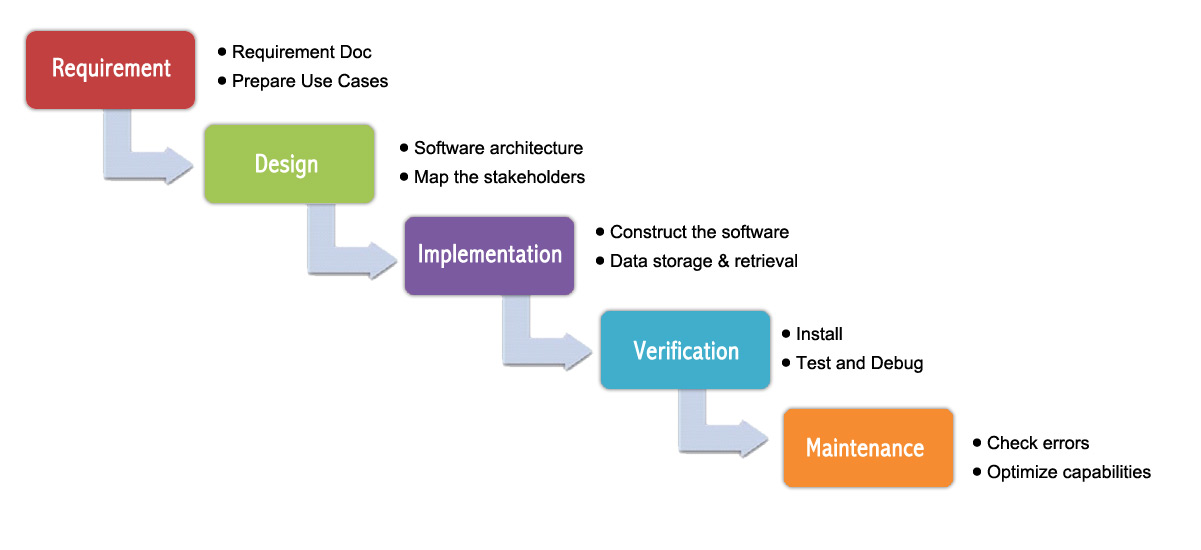
\includegraphics[width=\textwidth]{Waterfall}
    \caption{Waterfall Process Model}
    \label{fig:waterfall}
\end{figure}

As this process is sequential, once a step has been completed, developers can’t go back to a previous step – not without scratching the whole project and starting from the beginning. There is no place for change or error, so a project outcome and an extensive plan must be set in the beginning and then followed carefully, and for that reason overlapping is typically impossible in this methodology.
In waterfall methodologies all the requirements gathering and design work is done before any coding takes place.
 
Despite the success of the model in large and complex projects, it has a number of drawbacks like inflexibility, huge processes and the associated documentations irrespective of the size of the project \cite{method:Tommy2016}. A brief description of the advantages and disadvantages of this methodology is given bellow:\\

\textbf{Advantages of the Waterfall Methodology}
\begin{itemize}

\item Potential issues that would have been found during development can be researched and treated during the design phase, meaning that an alternate solution is selected before any code is written. Developers and customers agree on what will be delivered early in the development lifecycle making planning and designing more straightforward.\\

\item The development process tends to be better documented due to the fact that this methodology places greater emphasis on documentation, like requirements and design documents, being useful for many organizations.\\

\item The software can be designed completely and more carefully, based on a more complete understanding of all software deliverables. This provides a better software design with less likelihood of the “piecemeal effect”, a development phenomenon that can occur as pieces of code are defined and subsequently added to an application without knowing if they may or may not fit well \cite{waterfall:piecemeal}.
\end{itemize}

\textbf{Disadvantages of the Waterfall Methodology}
\begin{itemize}
\item If a set of change requests are introduced into the product while is undergoing testing, pausing the testing phase to do development is extremely heavy and expensive. So going back to a previous phase of the product's lifecycle is always a challenge.\\

\item It is not the best approach for large and complicated projects, where requirements may be frequently in change.\\

\item Since testing is one of the last phases in waterfall methodology, identifying risks and challenges in the earlier phases, and preparing a risk mitigation strategy, always become challenging.\\

\end{itemize}

\subsection{Agile Methodology}
Agile methodologies were developed to overcome the limitations of the Waterfall methodology. Instead of extensive planning and design up front, agile follows an incremental and iterative approach to development, where requirements and solutions evolve through collaboration between self-organizing, cross-functional teams - incorporating planners, designers, developers and testers - and customer. The Agile development refers to any development process that is aligned with the concepts of Agile Manifesto that says \cite{agile:manifesto}:\\

\textit{"We are uncovering better ways of developing software by doing it and helping others do it. We value:}

\begin{itemize}
\item \textit{Individuals and interactions over processes and tools.}
\item \textit{Working software over comprehensive documentation.}
\item \textit{Customer collaboration over contract negotiation.}
\item \textit{Responding to change over following a plan.}
\end{itemize}

The main goal of agile methodologies is the implementation of a project management process that encourages frequent inspection and adaption, leading to a set of engineering best practices in order to provided a rapid delivery of high-quality software, and also a business approach that aligns development with customer needs and company goals.
The main features of the most known agile methodologies are described below.
\subsubsection{Scrum}

is an iterative and incremental agile software development framework that makes use of software patterns, that are useful for project development in short time and where requirements are constantly in change. The scrum model comprises the existence of a series of iterations, also called Sprints, that are time-boxed which means that the duration is fixed, normally between 2 and 4 weeks, with two weeks being the most common. 

\begin{figure}[h]
    \centering
    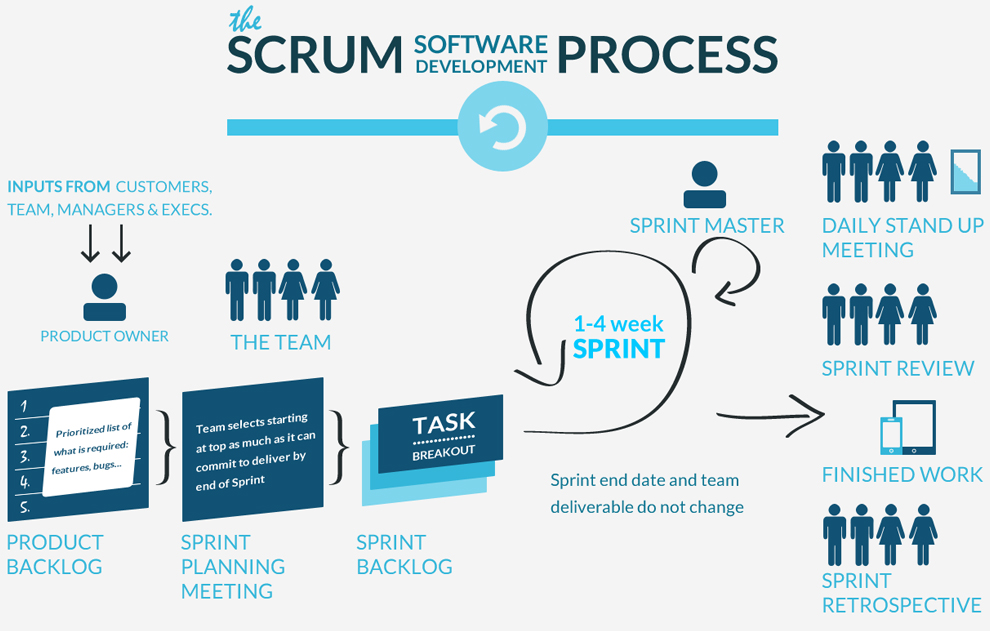
\includegraphics[width=0.9\textwidth]{scrumDevelopment}
    \caption{Scrum Software Development Process}
    \label{fig:waterfall}
\end{figure}

The process starts with the Product Catalog, where the product owner, which represents the stakeholders and customers, is responsible for understanding business and market requirements, and based on that creates a prioritized list of software requirements, and adds them to the Product Catalog. The Product owner maintains the Product Backlog up to date and at the quality level that the project team requires.

After that, a planning meeting is created, where the tasks for each sprint are identified in a form of Sprint Backlog and an estimated commitment for the sprint goal is made, followed by a review meeting, where the progress is reviewed and adjustments to be done in the next sprint are identified.

Each day during the sprint, the project team has a meeting, also called Daily Scrum, where each member gives feedback about what have been done since the last meeting, the current challenges and what is expected to be done until the next meeting.

Scrum is controlled by a Scrum Master, who is responsible for making the process run smoothly, for removing obstacles that impact productivity, and for organizing and facilitating the critical meetings. 

At the end of a sprint, the team conducts a sprint review during which the team demonstrates the new functionality to the product owner or any other stakeholder who wishes to provide feedback that could influence the next sprint.
Another activity in scrum project management is the sprint retrospective at the end of each sprint. The whole team participates in this meeting, including the Scrum Master and Product Owner. The meeting is an opportunity to reflect on the sprint that has ended, and identify opportunities to improve \cite{agile:scrum}.

\subsubsection{Extreme Programming (XP)}

is a software development methodology whose main goal is to improve software quality and responsiveness to changing customer requirements. 
XP uses an object-oriented approach as its paradigm of
drawing. The process consists of four activities: Planning, Project,
Encoding and Testing, which are repeated iterating through iteration.
Planning: It is created by the client, a set of stories that
Describe features and functionalities necessary for the software to be
built. Each story gives input to the methodology control system and is
Indexed and the client assigns it a priority value. Team members
Analyze this list and assign it costs if the story requires more than three
The client is asked to divide it. New stories can be added
any time. The next step is the team in collaboration with the customer
Decide which stories will get ready in the next iteration and on what date.
Project: The inherent philosophy is KIS (keep it simple), it is discouraged
Extra functionality because the developer
Thinks that later should be accurate. Often prototypes are generated,
Part of the project or of the whole. XP encourages
Refraction, a construction / design technique. (It is the process of changing and
Improve the internal software system, without altering the behavior
external.)
Encoding: Before the code, it recommends the process, that a
Battery of unit tests so that the story is satisfied. Then the focus of the
Programmers is the satisfaction of these unit tests. For coding XP,
Recommends that it be done in pairs. (Two heads work better than
), This guarantees other aspects such as quality, and speed (there is some
Scientific work that bought it to work in pairs, does not
Referring to Fig.
Yield, on the contrary usually more productivity is achieved).
Test: Unit tests are maintained over the various iterations and
Become part of a battery of regression tests, which is no longer
That all unit tests grouped together to be periodically tested for
Once in short periods (can be hours, at the end of the day, end of the week).
The idea is to confirm that nothing has stopped working.


blkabajkdkhakjsajdadads

\subsubsection{Feature Driven Development ( FDD )}
\subsubsection{Dynamic Systems Development Method ( DSDM) }
-------------------\\



Pros of Agile methods

Working software is delivered much more quickly and successive iterations can be delivered frequently, at a consistent pace.
There is closer collaboration between developers and the business.
Changes to requirements can be incorporated at any point of the process – even late in development.
It gives the opportunity for continuous improvement for live systems
It is highly transparent

Cons of Agile methods

Agile methodologies (e.g. Scrum, XP, Kanban, Crystal etc) are often more difficult to understand than linear, sequential ones – at least initially.
Because of the emphasis on working software there can be a perception that documentation can sometimes be neglected. The focus should be on appropriate documentation to the audience that needs it but, if not implemented well, this isn’t always the case.
When implemented badly Agile can introduce extra inefficiencies in large organisations or can be working against long standing organisational processes.



%%%%%%%%%%%%%%%%%%%%%%%%%%%%%%%%%%%%%%%%%%%%%%%%%%%%%%%%%%%%%%%%%%%%%%%%%%%%%%%
\section{Overview of The Proposal}\label{sec:evaluation}

%
%Works on MiKTeX only
%hint by http://goemonx.blogspot.de/2012/01/pdflatex-ligaturen-und-copynpaste.html
%also http://tex.stackexchange.com/questions/4397/make-ligatures-in-linux-libertine-copyable-and-searchable
%This allows a copy'n'paste of the text from the paper
\input glyphtounicode.tex
\pdfgentounicode=1

This section provides an overview of same major contributions in this area. Section 2.1 provides an insight about the core concepts of cloud computing, such as the architectural and business models of cloud computing. Section 2.2 describes some open standards related to the authentication and authorization protocols. Finally, Section 2.3 provides a comparison between the most known cloud storage providers and their services, including features and prices.
\subsection{Cloud Computing Core Concepts}\label{ssec:tools}
%%%%%%%%%%%%%%%%%%%%%%%%%%%%%%%%%%%%%%%%%%%%%%%%%%%%%%%%%%%%%%%%%%%%%%%%%%%%%%%

Described by the National Institute of Standards and Technology (NIST) as a {\it model for enabling convenient, on-demand network access to a shared pool of configurable computing resouces (e.g., networks, servers, storage, applications, and services) that can be rapidly provisioned and released with minimal management effort or service provider interaction}, \cite{Zhang2010}
cloud provides an architecture that can be divided into 4 layers: the hardware layer, the infrastructure layer, the platform and the application layer, as described bellow:

\begin{itemize}
\item \textit{The hardware layer}\\
Typically implemented in data centers, is responsible for managing the physical resources of the cloud, such as physical servers, routers, switches, power and cooling systems. Typical issues at hardware layer include hardware configuration, fault tolerance and traffic and power management.\cite{cloud:SS}\\

\item \textit{The infrastructure layer}\\
The infrastructure layer creates a pool of storage and computing resources by partitioning the physical resources using virtualization technologies (e.g., KVM, Xen, VMWare). It is an essential component of cloud computing since may key features are only available through virtualization technologies.\cite{cloud:SS} \\

\item \textit{The platform layer}\\
The platform layer is composed of the operating systems and application frameworks. Built on top of the infrastructure layer, the platform tries to minimize the load of deploying applications directly into VM containers. One of the best examples is the Google App Engine that operates at the platform layer to provide API support for implementing storage, database and business logic of typical web applications.\cite{cloud:SS}\\

\item \textit{The application layer}\\
Located at the the highest level of the hierarchy, the application layer consists of the actual cloud applications that make use of automatic-scaling feature to achieve better performance, availability and lower operating cost.\cite{cloud:SS}
\end{itemize}

Cloud computing also employs a service business model where hardware and platform-level resources are provided as services on-demand. In fact, every layer describe in the architecture can be implemented as a service to the layer below. Due to this fact, cloud offers services  that can be assigned to each layer, and grouped into three categories: infrastructure as a service (IaaS), platform as a service (PaaS) and software as a service (SaaS).


\begin{itemize}
\item \textit{IaaS - Infrastructure as a Servive }\\
It refers to on-demand provisioning of infrastructural resources i.e. users can subscribe to their favorite computing infrastructures with specified requirements in terms of hardware configuration, software installation and data access. Examples of IaaS providers include Amazon EC2 \cite{iaas:AmazonEC2} , GoGrid \cite{iaas:GoGrid} and Flexiscale\cite{iaas:FlexiScale}.  \\


\begin{figure}[h]
    \centering
    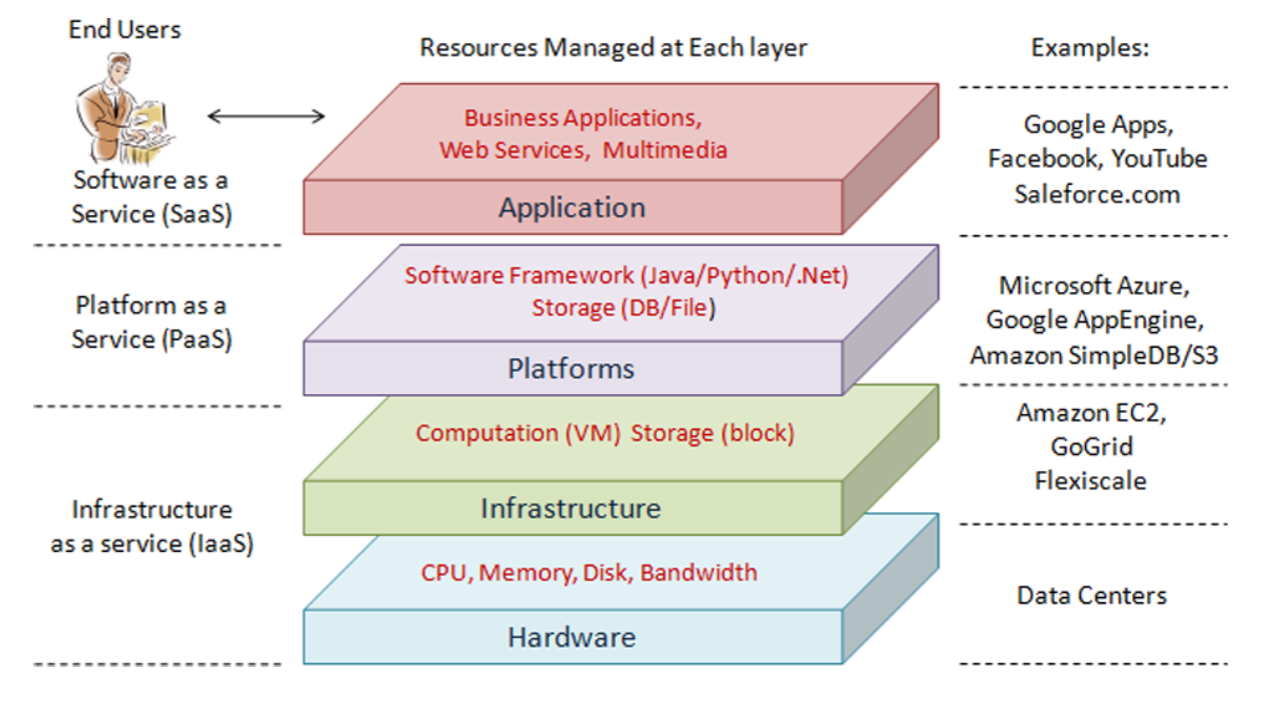
\includegraphics[width=\textwidth]{cloudArchitecture}
    \caption{Cloud Computing Architecture \cite{cloud:Archi}}
    \label{fig:cloudArchitecture}
\end{figure}

\item \textit{PaaS - Platform as a Servive }\\
It refers to the provisioning of platform software layer resources, including operating system support and software development frameworks. Examples of PaaS providers include Google App Engine, Microsoft Windows Azure and Force.com \cite{paas:Force}.\\

\item \textit{SaaS - Software as a Servive }\\
Software or an application is hosted as a service and provided to customers over the Internet. This is a very important service since it eliminates the need to install and run the application on the local computer. An important example of the SaaS is the Application Service Provider (ASP) whose main approach is to provide subscriptions to software that is hosted in the Internet. Google Chrome Browser is another example since it provides a desktop through which applications can be delivered locally or remotely, in addition to the traditional web browsing experience. Another examples include SalesForce.com and Rackspace \cite{saas:RackSpace}\\
\end{itemize}


\subsection{Web Authentication \& Authorization Open Technology}\label{ssec:security}


\begin{itemize}
\item {\it OpenID -} is an open standard for user authentication that allows the use of an existing account to sign in to multiple websites, without needing to create new passwords. It offers the possibility to associate information ( such as name or email address) with user's OpenID, that can be shared with the websites visited.

\begin{figure}[h]
    \centering
    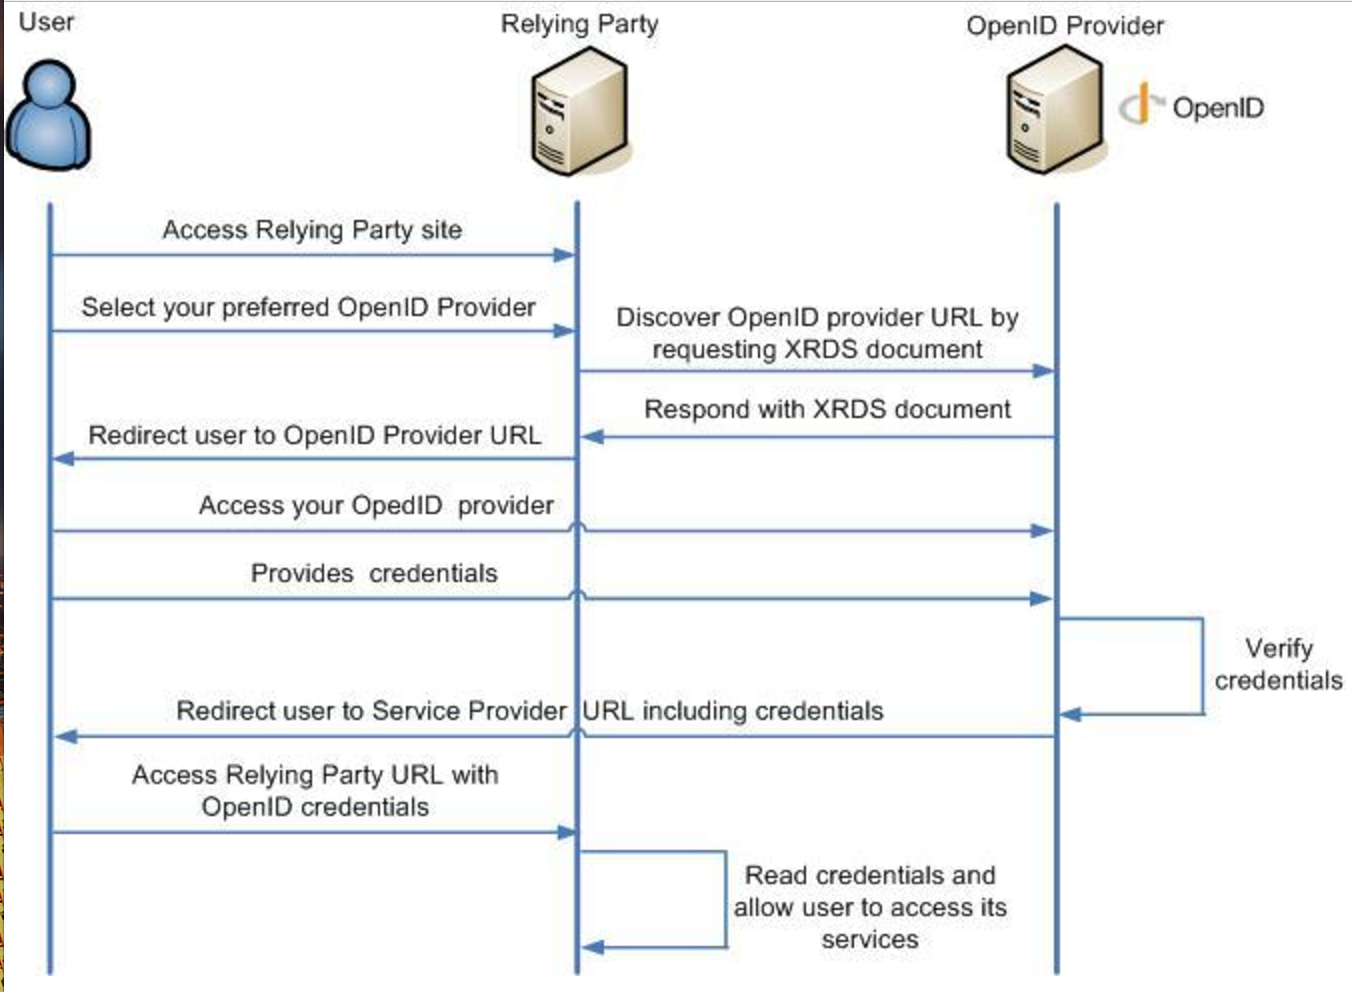
\includegraphics[width=1.0\textwidth]{openID}
    \caption{OpenID Authentication Flow}
    \label{fig:openID}
\end{figure}
%(citar o openID http://openid.net/get-an-openid/what-is-openid/).
To do that OpenID provides a framework for communication between the identity provider and the relying party. The user may have an account or multiple accounts with a specified identity provider, and then use this identity to authenticate to any service that accepts OpenID authentication. 

The flow process of OpenID comprises three entities: the user, the relying party which wants to verify the user identity and an entity provider that provides the OpenID URLs as despicted in figure \ref{fig:openID}.\\

With OpenID the user's password is only given to the identity provider and this one confirms the identity to the websites visited so, no website sees the password. Therefore, it is considered as safe since it not compromises the user's identity by some kind of insecure websites.\cite{cloud:openID}\\


\item {\it Shibboleth -} is another open standard, similar to OpenID, whose main approach is to manage single sign on (SSO), allowing users to authenticate to different services using just one piece of information.
Shibboleth is an open source implementation of federated identity based management, where the identity providers provide information and the service providers consume this information giving access to content or services. %{\textbf CITAR https://shibboleth.net/about/}. 

A user authenticates with his organizational credentials, and the organization (or identity provider) passes the minimal identity information necessary to the service provider to enable an authorization decision. It also provides extended privacy functionality allowing a user to control the attributes released to each application.\\ %{\textbf CITAR 15\\}


\item {\it OAuth - } is an open standard that provides a solution for internet users to authorize websites or applications to access their information, without sharing their credentials such as passwords or usernames.%\textbf {CITAR: Whitson Gordon. "Understanding OAuth: What Happens When You Log Into a Site with Google, Twitter, or Facebook". Retrieved 2016-05-15.}
Designed to work specifically with Hypertext Transfer Protocol (HTTP), it allows access tokens to be issued to third-party clients by an authorization server, with the approval of the resource owner. The third party then uses the access token to access the protected resources hosted by the resource server. %\textbf{CITAR: "RFC 6749 - The OAuth 2.0 Authorization Framework". Retrieved 2016-05-15.}

\begin{figure}[h]
    \centering
    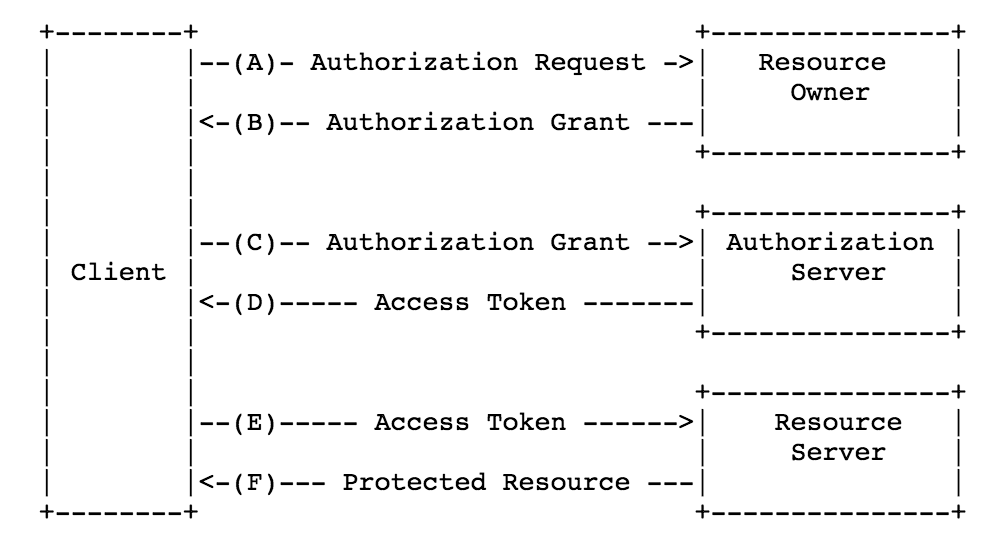
\includegraphics[width=1.0\textwidth]{OAuth}
    \caption{OAuth Protocol flow}
    \label{fig:OAuth}
\end{figure}

Since the creation, OAuth is being used by many social networking websites for authorization of various applications. Once the permissions are granted the application is able to download the complete stream of social data agains the user which is then kept for data mining purposes.% \textbf{CITAR O PAPER}.
More than a protocol, it is a framework is interoperable with any newer version of itself (e.g. Auth2.0).   
\end{itemize}

\subsection{Cloud Providers}\label{ssec:storage}

The industry of cloud storage has lot of potential in terms of growth of storage and faster retrieval. When organizations call for certain services offered by Cloud Storage Providers (CSPs), it is implicit that the they will choose the CSP that best suits the requirements of such organization. CSPs are also defined as Hosts, responsible for keeping the data available and accessible in a physical environment protected and running. People and organizations buy or lease storage capacity from the storage provider in order to store user, organization, or application data. Cloud storage Services may be accessed through cloud computer service, a web service application programming interface (API) or by applications that utilize the API, such as cloud desktop storage, a cloud storage gateway \cite{cloud:cloudStorageGateway} or Web-based content management systems.

Many cloud storage services offers a free account with some limitations, such as the amount of storage provided (usually from 2GB up to 5GB), or a file size limit for upload. 
An overview of the services  of the dominant Cloud Providers in the industry and their services is given bellow. 

\begin{enumerate}
\item {\it Amazon Cloud Drive -}
Amazon Cloud Drive is a cloud storage application managed by Amazon that offers secure cloud storage, file backup, file sharing and photo printing. Acting like a personal hard drive in the cloud, it can be accessed through multiple devices and offers 2 types of plans: one enables user with an unlimited storage for photos and the other one offers a 5GB of cloud storage space free of cost in a three-month trial.
There is no limit for the number of files to be uploaded, but each file needs to be under 2GB.

The advantage of Amazon Cloud Drive resides on the fact that if the user already have an Amazon account, doesn't need to sign up for a new service.
However, unlike other cloud storage services, the desktop app just allows the user to upload or download files, and can only view or manage files from the cloud drive website.\\

\item {\it Dropbox -}
Dropbox is one of the most used cloud storage services, allowing the store of any kind of file in the cloud. With Dropbox, users can easily move files from their computers to the cloud and vice versa by dragging and dropping them into the Dropbox folder.
The service automatically and quickly syncs files across all the devices registered for a specified account, available everywhere and independent from the device that it is being used. 
There is no size limit on file upload, but larger files can take several hours to upload, depending on network connection speed.
As an advantage, Dropbox gives its users a lot of opportunities to get extra storage (despite the 2GB offered through the sign up). If the user participate in the quick Getting Started Tutorial, the space increases more 250MB. Turn on the automatic photo upload feature on any of the mobile apps allows more 3GB of extra space. It's also possible to earn 500MB for each friend referred to Dropbox if it actually signs up for the service, up to 16GB total, or 32 referrals.
However, the website does not allow user to control how files are displayed.\\

\item {\it Box -}
Box is another cloud storage service that also provides sharing and privacy features for business and users. Beyond the basic cloud storage setup, where it's possible to store any kind of file, Box lets users to share files between them, assign tasks, leave comments on someone's work and get notifications when a file changes. User can also preview files from Box website and even create simple text documents. Like other cloud storage services box gives a lot of control over the privacy of a file, allowing user to decide who can view and open specific folders and files. It also allows user to define passwords for his files and set expiration dates for shared folders.
One of biggest advantages of Box is that, it allows business users to connect 
other apps, such as Salesforce and NetSuite \cite{cloud:netSuite}, so that you can easily save documents to Box. There are also plug-ins for Microsoft Office and Adobe Lightroom that let the user open and edit files saved to Box from those applications.

However The service's endless list of sharing and privacy features can be lost on someone who's just using the service for personal storage.
Because of all those features, it can feel overwhelming to navigate the Box website if you're only trying to manage a few files and folders.\\

\item {\it Microsoft OneDrive -}
OneDrive is a cloud storage service provided by Microsoft, that allows the store of any kind of file in the service, including photos, video and documents, and then access them from any Windows desktop or mobile device. One of the most important strengths of OneDrive, is that it works closely with Microsoft Office apps (e.g. Office 365). Therefore, anyone that has an Office 365 subscription will have access to OneDrive, collaborating with other people in real time.

In late 2015, Microsoft made an announcement that it would no longer offer unlimited cloud storage to Office 365 subscribers. Instead, subscribers are limited to 1TB. In the case of OneDrive Storage plans it offers a 50GB for \$1.99 per month plan (besides the 5GB offered initially to anyone that has a Microsoft Account). 
Another disadvantage of OneDrive resides on the fact that, the automatic file organization not always put files in the correct folders.\\

\item {\it Google Drive -}
Google Drive is the cloud storage service created by Google. Released on April 2012, allows users to store files in the cloud, synchronize files across devices and share files. It also combines a complete set of office tools such Google Docs, Sheets and Slides in an office suite that provides collaborative editing of documents, spreadsheets and presentations.
For those who have a Google account, it's easy to access google drive and enable the service in seconds. However, the 15GB initially provided are shared with other services such as Gmail (it's possible to save attachments from the e-mail directly to drive), and Google+. Like the other cloud providers, google drive can be accessed through a web browser or desktop app, but unfortunately if the user uses Google Drive tools to create documents, spreadsheets or presents, it must export those files to edit them in another program.
\end{enumerate}
The following table provides an overview of all the cloud providers described above and makes a comparison between them in terms of file size restriction, free storage, the possibility of earn extra storage, the paid plans that are available in the market and specific costs and the operative systems that supports each kind of service.
\begin{center}
\begin{tabular}{ |M{2.5cm}|M{2cm}|M{2cm}|M{2cm}|M{2cm}|M{2cm}|M{2cm}| }
 \hline
 \multicolumn{6}{|c|}{\textbf{Cloud Providers Comparison}} \\
 \hline
 & \textbf{OneDrive} & \textbf{Dropbox} & \textbf{Google Drive} & \textbf{Box} & \textbf{Amazon Cloud Drive}\\
 \hline
 \textbf{File Size Restriction} & 10GB&10GB with website, none with Dropbox apps&5TB&250MB for free plan, 5GB for paid personal plan&2GB*\\  \hline
 \textbf{Free storage} & 5GB&2GB&15GB&10GB&No**\\  \hline
 \textbf{Earn extra free storage} & No & Yes & No & No & No\\ \hline
 \textbf{Paid Plans} & €2/month for 50GB & €8.25/month for 1TB, €10/month unlimited storage for business teams (each user)	& €2/month 100GB, €10/month for 1TB up to 30TB of storage & €10/month for 100GB & €10.99/year for unlimited photos, €60/year for unlimited storage\\ \hline
 \textbf{OSes supported}	 & Windows, Mac, Android, iOS, Windows Phone	& Windows, Mac, Linux, Android, iOS, Windows Phone, BlackBerry, Kindle Fire	&Windows, Mac, Android, iOS	&Windows, Mac, Android, iOS, Windows Phone, BlackBerry	& Windows, Mac, Android, iOS, Kindle Fire.
\\
 \hline
\end{tabular}
*There is no file size limit with desktop apps.\\
**Amazon Cloud Drive offers limited free storage with an Amazon Prime subscription.
\end{center}





%%%%%%%%%%%%%%%%%%%%%%%%%%%%%%%%%%%%%%%%%%%%%%%%%%%%%%%%%%%%%%%%%%%%%%%%%%%%%%%

\section{Evaluation}\label{sec:schedule}

%
%Works on MiKTeX only
%hint by http://goemonx.blogspot.de/2012/01/pdflatex-ligaturen-und-copynpaste.html
%also http://tex.stackexchange.com/questions/4397/make-ligatures-in-linux-libertine-copyable-and-searchable
%This allows a copy'n'paste of the text from the paper
\input glyphtounicode.tex
\pdfgentounicode=1

This section provides an overview of same major contributions in this area. Section 2.1 provides an insight about the functional aspects of cloud, such as the architectural, business and various operation models of cloud computing. Section 2.2 describes some open standards related to the authentication and authorization protocols . Section 2.3 provides a brief introduction of the various cloud service providers and their services. FALTA COMPLETAR.... 
\section{Google em detalhe}
\section{Guidelines/Agile profile para fazer um protocolo web}\label{ssec:tools}




\subsection{Class Diagram}
\subsection{Functional Requirements}
\subsection{Technologies}
\subsubsection{Google API}
\subsubsection{Google API Spreadsheet}
\subsubsection{Node.js}
\subsubsection{Angular.js}



%%%%%%%%%%%%%%%%%%%%%%%%%%%%%%%%%%%%%%%%%%%%%%%%%%%%%%%%%%%%%%%%%%%%%%%%%%%%%%%

\section{Scheduling of Future Work}\label{sec:schedule}

%
%Works on MiKTeX only
%hint by http://goemonx.blogspot.de/2012/01/pdflatex-ligaturen-und-copynpaste.html
%also http://tex.stackexchange.com/questions/4397/make-ligatures-in-linux-libertine-copyable-and-searchable
%This allows a copy'n'paste of the text from the paper
\input glyphtounicode.tex
\pdfgentounicode=1

This section provides an overview of same major contributions in this area. Section 2.1 provides an insight about the functional aspects of cloud, such as the architectural, business and various operation models of cloud computing. Section 2.2 describes some open standards related to the authentication and authorization protocols . Section 2.3 provides a brief introduction of the various cloud service providers and their services. FALTA COMPLETAR.... 
\section{Google em detalhe}
\section{Guidelines/Agile profile para fazer um protocolo web}\label{ssec:tools}




\subsection{Class Diagram}
\subsection{Functional Requirements}
\subsection{Technologies}
\subsubsection{Google API}
\subsubsection{Google API Spreadsheet}
\subsubsection{Node.js}
\subsubsection{Angular.js}



%%%%%%%%%%%%%%%%%%%%%%%%%%%%%%%%%%%%%%%%%%%%%%%%%%%%%%%%%%%%%%%%%%%%%%%%%%%%%%%
\section{Conclusion}\label{sec:conclusion}

%
%Works on MiKTeX only
%hint by http://goemonx.blogspot.de/2012/01/pdflatex-ligaturen-und-copynpaste.html
%also http://tex.stackexchange.com/questions/4397/make-ligatures-in-linux-libertine-copyable-and-searchable
%This allows a copy'n'paste of the text from the paper
\input glyphtounicode.tex
\pdfgentounicode=1

This section provides an overview of same major contributions in this area. Section 2.1 provides an insight about the core concepts of cloud computing, such as the architectural and business models of cloud computing. Section 2.2 describes some open standards related to the authentication and authorization protocols. Finally, Section 2.3 provides a comparison between the most known cloud storage providers and their services, including features and prices.
\subsection{Cloud Computing Core Concepts}\label{ssec:tools}
%%%%%%%%%%%%%%%%%%%%%%%%%%%%%%%%%%%%%%%%%%%%%%%%%%%%%%%%%%%%%%%%%%%%%%%%%%%%%%%

Described by the National Institute of Standards and Technology (NIST) as a {\it model for enabling convenient, on-demand network access to a shared pool of configurable computing resouces (e.g., networks, servers, storage, applications, and services) that can be rapidly provisioned and released with minimal management effort or service provider interaction}, \cite{Zhang2010}
cloud provides an architecture that can be divided into 4 layers: the hardware layer, the infrastructure layer, the platform and the application layer, as described bellow:

\begin{itemize}
\item \textit{The hardware layer}\\
Typically implemented in data centers, is responsible for managing the physical resources of the cloud, such as physical servers, routers, switches, power and cooling systems. Typical issues at hardware layer include hardware configuration, fault tolerance and traffic and power management.\cite{cloud:SS}\\

\item \textit{The infrastructure layer}\\
The infrastructure layer creates a pool of storage and computing resources by partitioning the physical resources using virtualization technologies (e.g., KVM, Xen, VMWare). It is an essential component of cloud computing since may key features are only available through virtualization technologies.\cite{cloud:SS} \\

\item \textit{The platform layer}\\
The platform layer is composed of the operating systems and application frameworks. Built on top of the infrastructure layer, the platform tries to minimize the load of deploying applications directly into VM containers. One of the best examples is the Google App Engine that operates at the platform layer to provide API support for implementing storage, database and business logic of typical web applications.\cite{cloud:SS}\\

\item \textit{The application layer}\\
Located at the the highest level of the hierarchy, the application layer consists of the actual cloud applications that make use of automatic-scaling feature to achieve better performance, availability and lower operating cost.\cite{cloud:SS}
\end{itemize}

Cloud computing also employs a service business model where hardware and platform-level resources are provided as services on-demand. In fact, every layer describe in the architecture can be implemented as a service to the layer below. Due to this fact, cloud offers services  that can be assigned to each layer, and grouped into three categories: infrastructure as a service (IaaS), platform as a service (PaaS) and software as a service (SaaS).


\begin{itemize}
\item \textit{IaaS - Infrastructure as a Servive }\\
It refers to on-demand provisioning of infrastructural resources i.e. users can subscribe to their favorite computing infrastructures with specified requirements in terms of hardware configuration, software installation and data access. Examples of IaaS providers include Amazon EC2 \cite{iaas:AmazonEC2} , GoGrid \cite{iaas:GoGrid} and Flexiscale\cite{iaas:FlexiScale}.  \\


\begin{figure}[h]
    \centering
    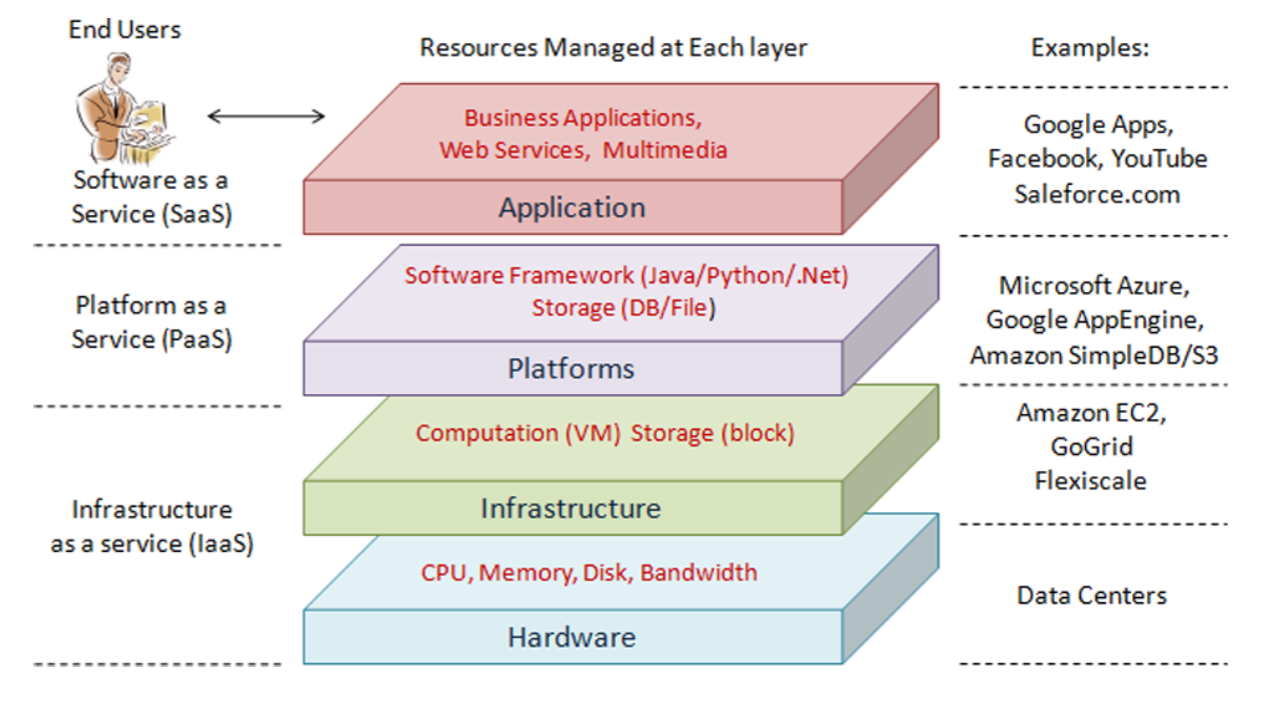
\includegraphics[width=\textwidth]{cloudArchitecture}
    \caption{Cloud Computing Architecture \cite{cloud:Archi}}
    \label{fig:cloudArchitecture}
\end{figure}

\item \textit{PaaS - Platform as a Servive }\\
It refers to the provisioning of platform software layer resources, including operating system support and software development frameworks. Examples of PaaS providers include Google App Engine, Microsoft Windows Azure and Force.com \cite{paas:Force}.\\

\item \textit{SaaS - Software as a Servive }\\
Software or an application is hosted as a service and provided to customers over the Internet. This is a very important service since it eliminates the need to install and run the application on the local computer. An important example of the SaaS is the Application Service Provider (ASP) whose main approach is to provide subscriptions to software that is hosted in the Internet. Google Chrome Browser is another example since it provides a desktop through which applications can be delivered locally or remotely, in addition to the traditional web browsing experience. Another examples include SalesForce.com and Rackspace \cite{saas:RackSpace}\\
\end{itemize}


\subsection{Web Authentication \& Authorization Open Technology}\label{ssec:security}


\begin{itemize}
\item {\it OpenID -} is an open standard for user authentication that allows the use of an existing account to sign in to multiple websites, without needing to create new passwords. It offers the possibility to associate information ( such as name or email address) with user's OpenID, that can be shared with the websites visited.

\begin{figure}[h]
    \centering
    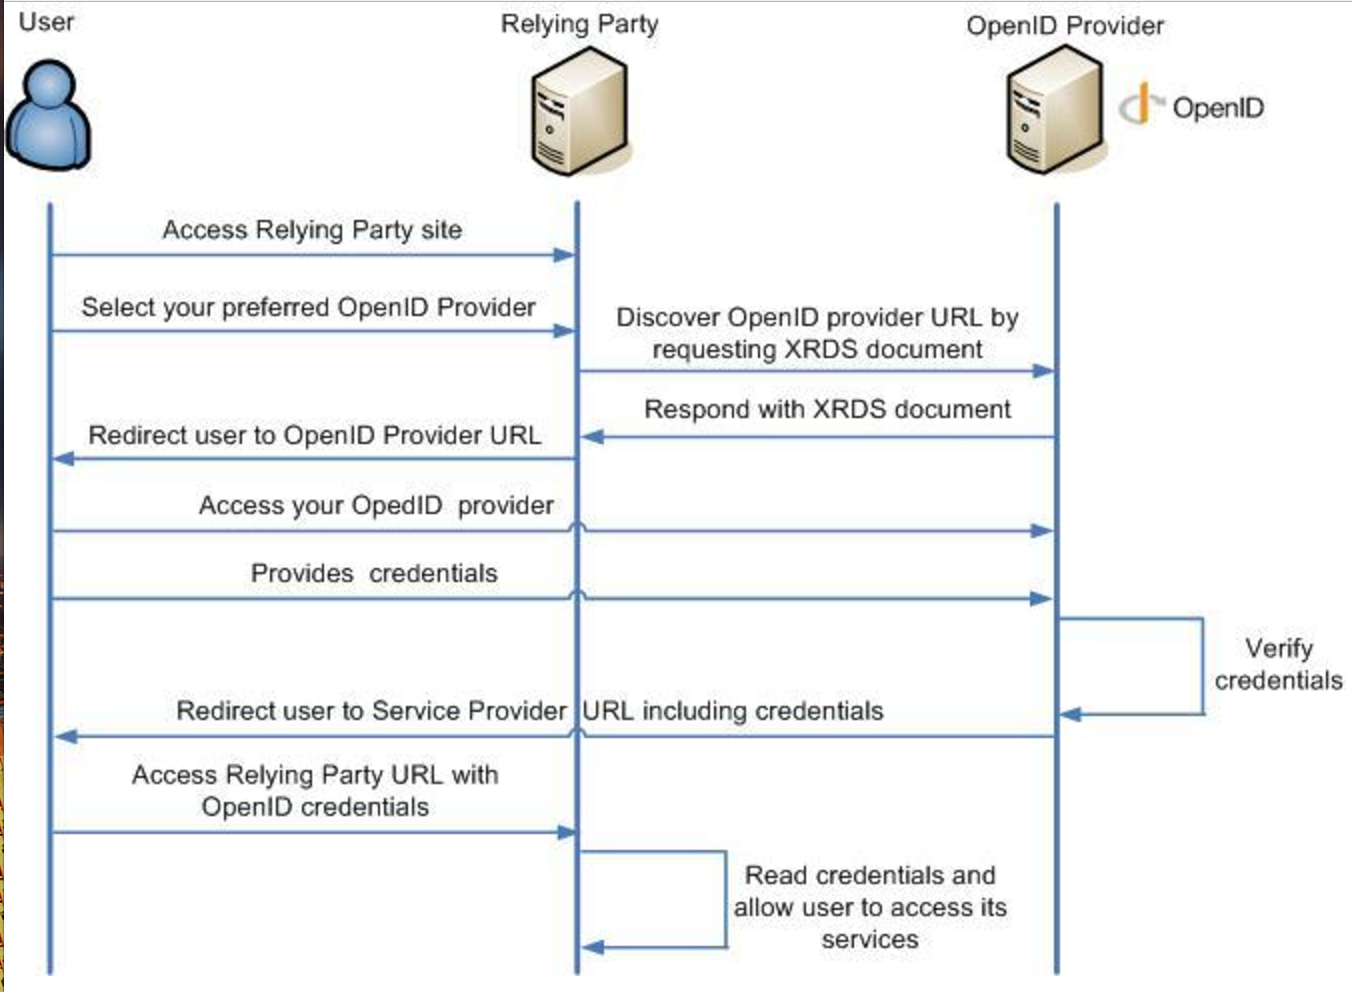
\includegraphics[width=1.0\textwidth]{openID}
    \caption{OpenID Authentication Flow}
    \label{fig:openID}
\end{figure}
%(citar o openID http://openid.net/get-an-openid/what-is-openid/).
To do that OpenID provides a framework for communication between the identity provider and the relying party. The user may have an account or multiple accounts with a specified identity provider, and then use this identity to authenticate to any service that accepts OpenID authentication. 

The flow process of OpenID comprises three entities: the user, the relying party which wants to verify the user identity and an entity provider that provides the OpenID URLs as despicted in figure \ref{fig:openID}.\\

With OpenID the user's password is only given to the identity provider and this one confirms the identity to the websites visited so, no website sees the password. Therefore, it is considered as safe since it not compromises the user's identity by some kind of insecure websites.\cite{cloud:openID}\\


\item {\it Shibboleth -} is another open standard, similar to OpenID, whose main approach is to manage single sign on (SSO), allowing users to authenticate to different services using just one piece of information.
Shibboleth is an open source implementation of federated identity based management, where the identity providers provide information and the service providers consume this information giving access to content or services. %{\textbf CITAR https://shibboleth.net/about/}. 

A user authenticates with his organizational credentials, and the organization (or identity provider) passes the minimal identity information necessary to the service provider to enable an authorization decision. It also provides extended privacy functionality allowing a user to control the attributes released to each application.\\ %{\textbf CITAR 15\\}


\item {\it OAuth - } is an open standard that provides a solution for internet users to authorize websites or applications to access their information, without sharing their credentials such as passwords or usernames.%\textbf {CITAR: Whitson Gordon. "Understanding OAuth: What Happens When You Log Into a Site with Google, Twitter, or Facebook". Retrieved 2016-05-15.}
Designed to work specifically with Hypertext Transfer Protocol (HTTP), it allows access tokens to be issued to third-party clients by an authorization server, with the approval of the resource owner. The third party then uses the access token to access the protected resources hosted by the resource server. %\textbf{CITAR: "RFC 6749 - The OAuth 2.0 Authorization Framework". Retrieved 2016-05-15.}

\begin{figure}[h]
    \centering
    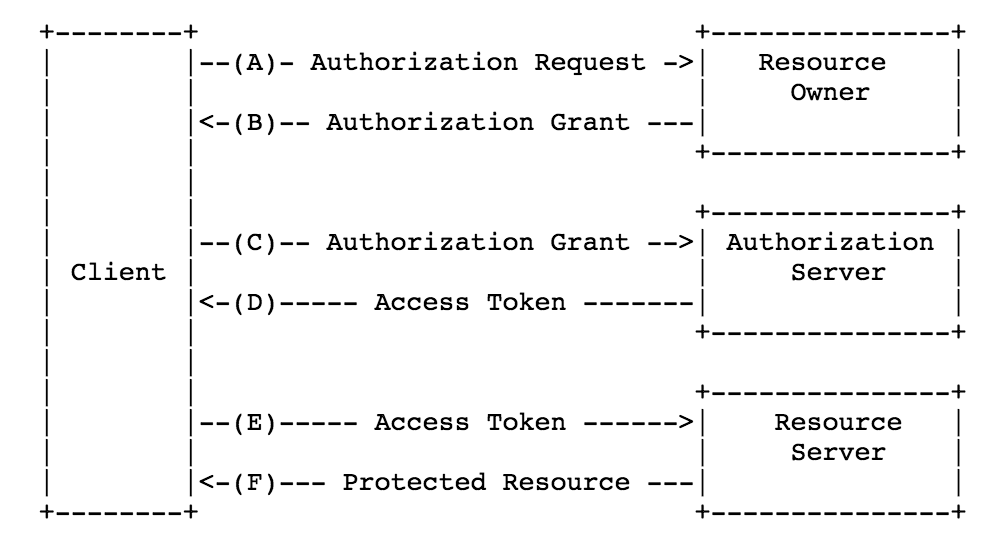
\includegraphics[width=1.0\textwidth]{OAuth}
    \caption{OAuth Protocol flow}
    \label{fig:OAuth}
\end{figure}

Since the creation, OAuth is being used by many social networking websites for authorization of various applications. Once the permissions are granted the application is able to download the complete stream of social data agains the user which is then kept for data mining purposes.% \textbf{CITAR O PAPER}.
More than a protocol, it is a framework is interoperable with any newer version of itself (e.g. Auth2.0).   
\end{itemize}

\subsection{Cloud Providers}\label{ssec:storage}

The industry of cloud storage has lot of potential in terms of growth of storage and faster retrieval. When organizations call for certain services offered by Cloud Storage Providers (CSPs), it is implicit that the they will choose the CSP that best suits the requirements of such organization. CSPs are also defined as Hosts, responsible for keeping the data available and accessible in a physical environment protected and running. People and organizations buy or lease storage capacity from the storage provider in order to store user, organization, or application data. Cloud storage Services may be accessed through cloud computer service, a web service application programming interface (API) or by applications that utilize the API, such as cloud desktop storage, a cloud storage gateway \cite{cloud:cloudStorageGateway} or Web-based content management systems.

Many cloud storage services offers a free account with some limitations, such as the amount of storage provided (usually from 2GB up to 5GB), or a file size limit for upload. 
An overview of the services  of the dominant Cloud Providers in the industry and their services is given bellow. 

\begin{enumerate}
\item {\it Amazon Cloud Drive -}
Amazon Cloud Drive is a cloud storage application managed by Amazon that offers secure cloud storage, file backup, file sharing and photo printing. Acting like a personal hard drive in the cloud, it can be accessed through multiple devices and offers 2 types of plans: one enables user with an unlimited storage for photos and the other one offers a 5GB of cloud storage space free of cost in a three-month trial.
There is no limit for the number of files to be uploaded, but each file needs to be under 2GB.

The advantage of Amazon Cloud Drive resides on the fact that if the user already have an Amazon account, doesn't need to sign up for a new service.
However, unlike other cloud storage services, the desktop app just allows the user to upload or download files, and can only view or manage files from the cloud drive website.\\

\item {\it Dropbox -}
Dropbox is one of the most used cloud storage services, allowing the store of any kind of file in the cloud. With Dropbox, users can easily move files from their computers to the cloud and vice versa by dragging and dropping them into the Dropbox folder.
The service automatically and quickly syncs files across all the devices registered for a specified account, available everywhere and independent from the device that it is being used. 
There is no size limit on file upload, but larger files can take several hours to upload, depending on network connection speed.
As an advantage, Dropbox gives its users a lot of opportunities to get extra storage (despite the 2GB offered through the sign up). If the user participate in the quick Getting Started Tutorial, the space increases more 250MB. Turn on the automatic photo upload feature on any of the mobile apps allows more 3GB of extra space. It's also possible to earn 500MB for each friend referred to Dropbox if it actually signs up for the service, up to 16GB total, or 32 referrals.
However, the website does not allow user to control how files are displayed.\\

\item {\it Box -}
Box is another cloud storage service that also provides sharing and privacy features for business and users. Beyond the basic cloud storage setup, where it's possible to store any kind of file, Box lets users to share files between them, assign tasks, leave comments on someone's work and get notifications when a file changes. User can also preview files from Box website and even create simple text documents. Like other cloud storage services box gives a lot of control over the privacy of a file, allowing user to decide who can view and open specific folders and files. It also allows user to define passwords for his files and set expiration dates for shared folders.
One of biggest advantages of Box is that, it allows business users to connect 
other apps, such as Salesforce and NetSuite \cite{cloud:netSuite}, so that you can easily save documents to Box. There are also plug-ins for Microsoft Office and Adobe Lightroom that let the user open and edit files saved to Box from those applications.

However The service's endless list of sharing and privacy features can be lost on someone who's just using the service for personal storage.
Because of all those features, it can feel overwhelming to navigate the Box website if you're only trying to manage a few files and folders.\\

\item {\it Microsoft OneDrive -}
OneDrive is a cloud storage service provided by Microsoft, that allows the store of any kind of file in the service, including photos, video and documents, and then access them from any Windows desktop or mobile device. One of the most important strengths of OneDrive, is that it works closely with Microsoft Office apps (e.g. Office 365). Therefore, anyone that has an Office 365 subscription will have access to OneDrive, collaborating with other people in real time.

In late 2015, Microsoft made an announcement that it would no longer offer unlimited cloud storage to Office 365 subscribers. Instead, subscribers are limited to 1TB. In the case of OneDrive Storage plans it offers a 50GB for \$1.99 per month plan (besides the 5GB offered initially to anyone that has a Microsoft Account). 
Another disadvantage of OneDrive resides on the fact that, the automatic file organization not always put files in the correct folders.\\

\item {\it Google Drive -}
Google Drive is the cloud storage service created by Google. Released on April 2012, allows users to store files in the cloud, synchronize files across devices and share files. It also combines a complete set of office tools such Google Docs, Sheets and Slides in an office suite that provides collaborative editing of documents, spreadsheets and presentations.
For those who have a Google account, it's easy to access google drive and enable the service in seconds. However, the 15GB initially provided are shared with other services such as Gmail (it's possible to save attachments from the e-mail directly to drive), and Google+. Like the other cloud providers, google drive can be accessed through a web browser or desktop app, but unfortunately if the user uses Google Drive tools to create documents, spreadsheets or presents, it must export those files to edit them in another program.
\end{enumerate}
The following table provides an overview of all the cloud providers described above and makes a comparison between them in terms of file size restriction, free storage, the possibility of earn extra storage, the paid plans that are available in the market and specific costs and the operative systems that supports each kind of service.
\begin{center}
\begin{tabular}{ |M{2.5cm}|M{2cm}|M{2cm}|M{2cm}|M{2cm}|M{2cm}|M{2cm}| }
 \hline
 \multicolumn{6}{|c|}{\textbf{Cloud Providers Comparison}} \\
 \hline
 & \textbf{OneDrive} & \textbf{Dropbox} & \textbf{Google Drive} & \textbf{Box} & \textbf{Amazon Cloud Drive}\\
 \hline
 \textbf{File Size Restriction} & 10GB&10GB with website, none with Dropbox apps&5TB&250MB for free plan, 5GB for paid personal plan&2GB*\\  \hline
 \textbf{Free storage} & 5GB&2GB&15GB&10GB&No**\\  \hline
 \textbf{Earn extra free storage} & No & Yes & No & No & No\\ \hline
 \textbf{Paid Plans} & €2/month for 50GB & €8.25/month for 1TB, €10/month unlimited storage for business teams (each user)	& €2/month 100GB, €10/month for 1TB up to 30TB of storage & €10/month for 100GB & €10.99/year for unlimited photos, €60/year for unlimited storage\\ \hline
 \textbf{OSes supported}	 & Windows, Mac, Android, iOS, Windows Phone	& Windows, Mac, Linux, Android, iOS, Windows Phone, BlackBerry, Kindle Fire	&Windows, Mac, Android, iOS	&Windows, Mac, Android, iOS, Windows Phone, BlackBerry	& Windows, Mac, Android, iOS, Kindle Fire.
\\
 \hline
\end{tabular}
*There is no file size limit with desktop apps.\\
**Amazon Cloud Drive offers limited free storage with an Amazon Prime subscription.
\end{center}





%%%%%%%%%%%%%%%%%%%%%%%%%%%%%%%%%%%%%%%%%%%%%%%%%%%%%%%%%%%%%%%%%%%%%%%%%%%%%%%

%%%%%%%%%%%%%%%%%%%%%%%%%%%%%%%%%%%%%%%%%%%%%%%%%%%%%%%%%%%%%%%%%%%%%%%%%%%%%%%
\begin{thebibliography}{9}

\bibitem{cloud:tweaks} 
  CloudTweaks,
  Cloud Computing - Demystifying SAAS, PAAS AND IAAS,
  http://cloudtweaks.com/2010/05/cloud-computing-demystifying-saas-paas-and-iaas/,
  May 3,2010.
  
\bibitem{cloud:SS}
Nanyang Technological University, SINGAPORE (2010). Cloud computing: A perspective study. In New Generation Computing. 

\bibitem{Zhang2010}
Zhang, Q., Cheng, L., Boutaba, R. (2010). Cloud computing: State-of-the-art and research challenges. Journal of Internet Services and Applications.


\bibitem{iaas:AmazonEC2} 
Amazon Elastic Computing Cloud, aws.amazon.com/ec2,

\bibitem{iaas:GoGrid}
Cloud Hosting, CLoud Computing and Hybrid Infrastructure from GoGrid, http://www.gogrid.com

\bibitem{iaas:FlexiScale}
FlexiScale Cloud Comp and Hosting, www.flexiscale.com

\bibitem{paas:Force}
Salesforce CRM, http://www.salesforce.com/platform

\bibitem{saas:RackSpace}
Dedicated Server, Managed Hosting, Web Hosting by Rackspace Hosting, http://www.rackspace.com

\bibitem{cloud:openID}
The Foundation of Internet Identity, A very brief history of OpenID Connect, http://openid.net/get-an-openid/what-is-openid/

\bibitem{cloud:Archi}
Cloud, Networking \& Data Analytics,
All about cloud computing, networking and data, analytics, http://cloudcomputingnet.com/cloud-computing-architecture/

\bibitem{cloud:cloudStorageGateway}
Death of a middleman: Cloud storage gateways – and their evolution, http://www.theregister.co.uk/2015/05/25/cloud\_storage\_gateways/

\bibitem{cloud:netSuite}
NetSuite: Business Software, Business Management Software, http://www.netsuite.com/portal/home.shtml

\bibitem{agile:1}
 B. Bohem, “Making a difference in the software century,” IEEE Computer, pp. 78-84, Mar. 2008
 
\bibitem{method:Tommy2016}
Tommy, R., Mhaisekar, M., Kallepally, S., Varghese, L., Ahmed, S., \& Somaraju, M. D. (2016). Dynamic quality control in agile methodology for improving the quality. 2015 IEEE International Conference on Computer Graphics, Vision and Information Security, CGVIS 2015, 233–236.

\bibitem{waterfall:piecemeal}
 John Stark, Product Lifecycle Management: 21st Century Paradigm for Product Realisation, 2nd Edition,
 
\bibitem{agile:manifesto}
 Fowler, M., \& Highsmith, J. (2001). The agile manifesto. Software Development, 9(August), 28–35. 

\bibitem{agile:scrum}
Manuja, M. (2014). Moving agile based projects on Cloud. 2014 IEEE International Advance Computing Conference (IACC), 1392–1397. 

\end{thebibliography}

\bibliographystyle{splncs03}
\bibliography{paper}
%%%%%%%%%%%%%%%%%%%%%%%%%%%%%%%%%%%%%%%%%%%%%%%%%%%%%%%%%%%%%%%%%%%%%%%%%%%%%%%
\end{document}
